\section{Limitations of Existing Multipath Protocols}
A large number of researches~\cite{oh2016feedback,barik2016lisa,khalili2013mptcp,kheirkhah2016mmptcp,kheirkhah2015short} have explored MPTCP as an alternative of TCP for various application and network scenarios. However, MPTCP has two major shortcomings that prevent its large scale deployment over the Internet -- (a) MPTCP is implemented as a part of the Linux kernel, and therefore requires device reconfiguration for its deployment; and (b) MPTCP is still under exploration phase, and there are multiple shortcomings of MPTCP as pointed out by existing researches. In~\cite{khalili2013mptcp}, Khalili \textit{et al.} have claimed that MPTCP is not pareto optimal. Further, in~\cite{kheirkhah2016mmptcp}, the authors have pointed out that MPTCP is not suitable for short connections. On the other hand, MP-QUIC has been proposed recently to explore multipath capability over QUIC protocol~\cite{mpquic-measure}.
In this section, we first explore the performance of MPTCP and MP-QUIC over short lived flows. 

\subsection{MPTCP for Short Lived Flows} 
%For this, we ask the following question: \textit{Why does MPTCP perform poorly for short flows?}  To get the answer, 
To explore MPTCP for short lived flows, we conduct experiments with the help of \texttt{Mininet} environment\footnote{\url{http://mininet.org/} (last accessed: \today)}, where we setup a network with two multi-homed hosts with two distinct paths between them. We vary the round trip time (RTT) for the two paths, and then transfer data between the two hosts. For our experiment, we have configured the Linux kernel of the hosts with MPTCP version 0.91~\footnote{\url{http://multipath-tcp.org/} (last accessed: \today)}. We set the path bandwidth as $100$ Mbps. 
We keep a file at the server, and download that file from the client through MPTCP based connection. To observe the MPTCP behavior for various connection types, we vary the size of the file, and measure the impacts.

\begin{figure}[!t]
%	\captionsetup[subfigure]{}
	\begin{center}
		\begin{subfigure}{.46\linewidth}
			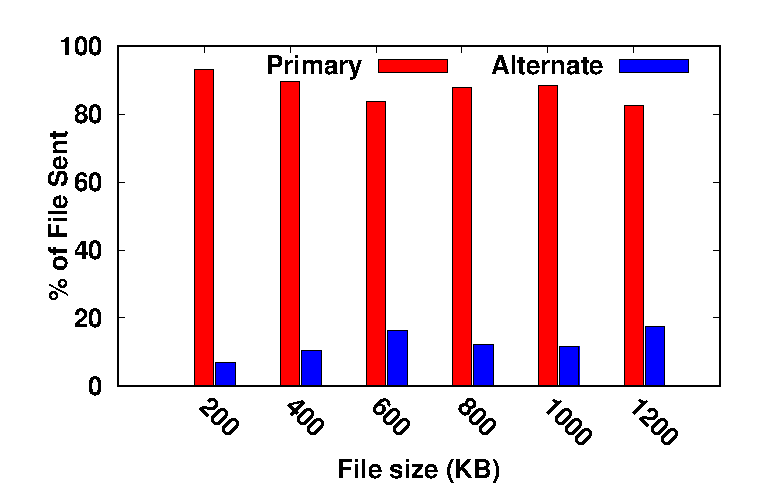
\includegraphics[width=0.95\linewidth]{img/exp4/delay-5}
			\caption{\label{fig:percentSentOverPathRTT80}RTT = 80ms}
		\end{subfigure}
		\hspace{0.1cm}
		\begin{subfigure}{.46\linewidth}
			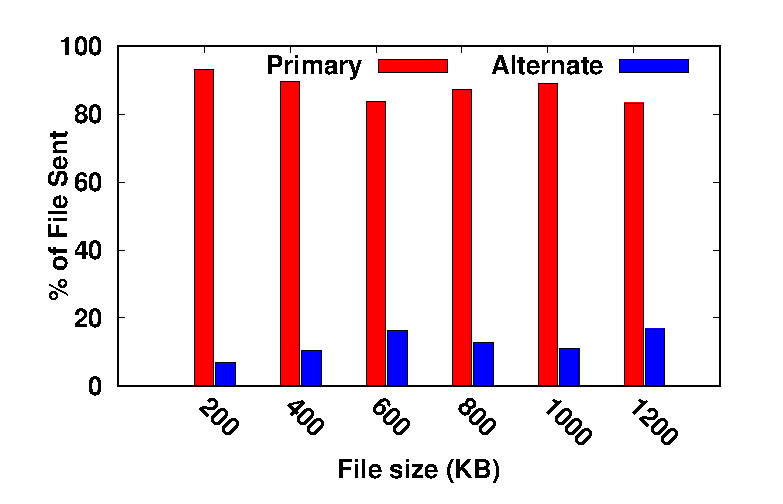
\includegraphics[width=0.95\linewidth]{img/exp4/delay-20}
			\caption{\label{fig:percentSentOverPathRTT320}RTT = 320ms}
		\end{subfigure}
		
		\caption{\label{fig:percentSentOverPath}Percentage of data share between the primary and the alternate paths}
	\end{center}
\end{figure}

\subsubsection{Utilization of Network Bandwidth at Alternate Paths for Short Flows}
MPTCP first initiates the connection through one of the available paths, called the {\em primary path}, and then explores the {\em alternate paths} to initiate alternate connections through them. In the first experiment, we try to look into the amount of data shares between the primary path and the alternate path. For this, we keep the bandwidth and latency for both the paths same, and vary the flow duration by increasing the size of the file to be downloaded at the client from the server. The results are plotted in Fig.~\ref{fig:percentSentOverPath}. We can observe from that figure that 
%there is a huge imbalance between the two paths in terms of data share. T
the primary path forwards significantly more data compared to the alternate path. By exploring the connection logs, we find that by the time MPTCP sets up a connection to the alternate path, most of the data for a short flow has been transferred over the primary path. Further, the congestion controls for the primary and the alternate paths are handled separately, and therefore the alternate path also needs to go through the slow start phase. 

\subsubsection{Impact of Path Selection for Connection Initiation}
We then perform another experiment on path selection, where the two paths have different RTT. Here, we explore the effect of primary path selection. 
Consequently, we vary the RTT of the two paths, and the results are plotted in Fig.~\ref{fig:timeSentOverPath}. The two different bars in the graphs show the average file download time for the two cases -- (i) the low RTT path is used as the primary path, and (ii) the high RTT path is used as the primary path. We observe that for small size file download, the performance varies a lot based on the selection of the primary path. 

\begin{figure}[!t]
%    \captionsetup[subfigure]{}
    \begin{center}
    	\begin{subfigure}{.46\linewidth}
    		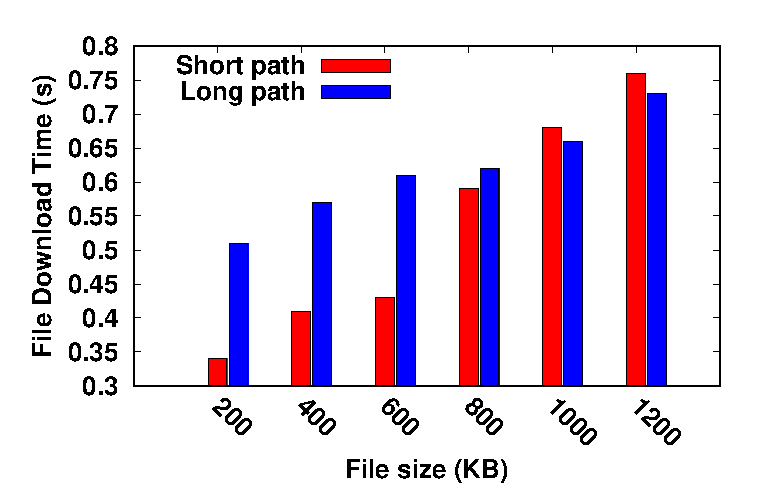
\includegraphics[width=0.95\linewidth]{img/exp5/time_needed_5}
    		\caption{\label{fig:timeSentOverPathRTT80}RTT: short path = 80ms, long path = 120ms}
    	\end{subfigure}
		\hspace{0.1cm}
		\begin{subfigure}{.46\linewidth}
			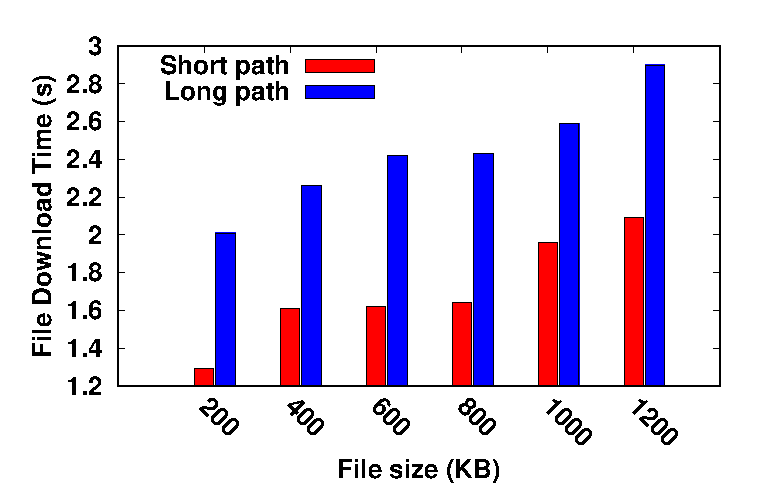
\includegraphics[width=0.95\linewidth]{img/exp5/time_needed_20}
			\caption{\label{fig:timeSentOverPathRTT320}RTT: short path = 320ms, long path = 480ms}
		\end{subfigure}
        
        \caption{\label{fig:timeSentOverPath} File download time when short path is the primary path vs when long path is the primary path}
    \end{center}
\end{figure}

\begin{figure}[!t]
%	\captionsetup[subfigure]{}
	\begin{center}
		\begin{subfigure}{.46\linewidth}
			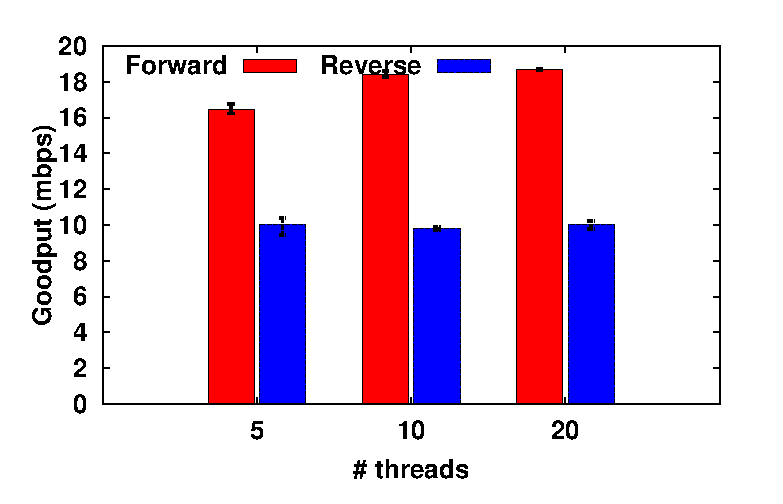
\includegraphics[width=0.95\linewidth]{img/mpquic-prob/goodPut-5.eps}
			\caption{\label{fig:Goodput-mpquic}Goodput}
		\end{subfigure}
		\hspace{0.1cm}
		\begin{subfigure}{.46\linewidth}
			\caption{\label{fig:flowcomplition-mpquic}Transmission complition time}
			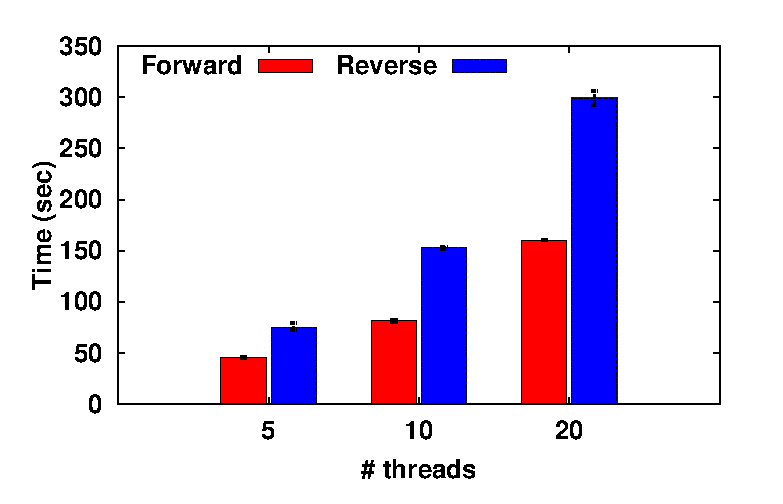
\includegraphics[width=0.95\linewidth]{img/mpquic-prob/tymdiff-5.eps}
		\end{subfigure}
		
		\caption{\label{fig:mpquic-back}}
	\end{center}
\end{figure}

\subsection{MP-QUIC for Short Lived Flows -- Impact on Flow Direction}
QUIC is a protocol to solve the issue of short lived communication. But it was not multi-path. So, Coninck {\em et. al.} developed MPQUIC to counter this problem~\cite{mpquic-measure}. However, as we discussed earlier that it depends on the devices routing policy and therefore may not work properly. We have performed few tests where one of the hosts have two interfaces (i.e. multi-homed host) while another have only one interface (single-homed host). The detailed experimental methodology and setup are given in Section~\ref{exp}.  When the data is transmitted from single-homed host to multi-homed host, we call it the forward traffic; similarly, while it is in other direction, we call it as reverse traffic. We have sent multiple back-to-back short flows through variable number of simultaneous threads in both direction. Fig.~\ref{fig:mpquic-back} represents a snapshot of the result we observed in this experiment.  Here we observe that, there is a huge difference in goodput\footnote{Transmission rate observed by an application i.e. it does not considered retransmissions.} as well as the connection completion time in between the forward and the reverse mode for MP-QUIC. This indicates that MP-QUIC is not always efficient in utilizing multiple paths.

\subsection{Take Aways}
In summary, the lessons learned from the above experiments are as follows. (a) \textbf{Connection establishment time is an overhead for short flows.} Further flow based congestion control algorithms result in the underutilization of network bandwidth, because every transport layer flow independently increases its transmission rate from the scratch (by increasing the congestion window value for TCP or MPTCP), and the flow may end before its transmission rate reaches to the network capacity. 
(b) \textbf{Connection establishment and path selection cannot be independent for a multi-path protocol}, because the performance depends on the path selection mechanism. We need to develop a mechanism where the data transmission can be initiated simultaneously at multiple paths.  
